\documentclass{article}
\usepackage[utf8]{inputenc}
\usepackage{amsmath}
\usepackage{amsthm}
\usepackage{amsfonts}
\usepackage{amssymb}
\usepackage[left=2cm,right=2cm,top=2cm,bottom=2cm,includeheadfoot]{geometry}
\usepackage{color}
\usepackage[format=hang]{caption}
\captionsetup[subtable]{justification=centering}
\usepackage{enumerate}
\usepackage{setspace}
\usepackage{hyperref}
\usepackage{footnote}
\usepackage{appendix}
\usepackage{subcaption}
\usepackage{graphicx}
\usepackage{bbm}
\usepackage{framed}
\usepackage{float}
\usepackage{listings}



\begin{document}



\section{Using get\_scenarios}

To get started you would include the package as so:\\

\begin{figure}[H]
	\begin{framed}
		import prescient\_gosm.get\_scenarios as get\_scenarios
	\end{framed}
\end{figure}

\paragraph{}
Whenever you want to create scenarios you would call the package's 'create\_scenarios' function. This function takes two dictionaries corresponding to the options for the scenario generation process as arguments. This is described more in the next section but for now know that Pop\_opts and SC\_opts are dictionaries. 


\begin{figure}[H]
	\begin{framed}
		get\_scenarios.generate(Pop\_opts, SC\_opts)
	\end{framed}
\end{figure}

\paragraph{}
This will generate the scenarios and place the relevant files in the output directory that was specified in the Pop\_opts dictionary. If you need the relative path to the output directory you can just assign the function to a value which will thus contain the path name.


\begin{figure}[H]
	\begin{framed}
		path\_to\_output = get\_scenarios.generate(Pop\_opts, SC\_opts)
	\end{framed}
\end{figure}

\section{Passing in Options}

\paragraph{}
We will now describe the dictionaries you are supposed to pass in for the get\_scenarios functions. The dictionaries contain a key for the option you would like to alter in string format and a corresponding value. If the value is not numerical or boolean it must be in string format. You will pass in two of these dictionaries. 

\begin{enumerate}
\item The first dictionary will correspond to the options passed into the populator options file. To learn more about every option available for the populator options refer to the gosm documentation. However, we will list the required options. Not including these options will result in an error, since these options are required.
\begin{itemize}
	\item \textbf{start-date \& end-date}: These dates determine the period for which scenarios are created. Both must be in the format of YYYY-MM-DD-HH:MM.
	\item \textbf{output-directory}: The path that stores the output.
	\item \textbf{sources-file}: The sourcelist file.
\end{itemize}
\begin{figure}[H]
	\centering
	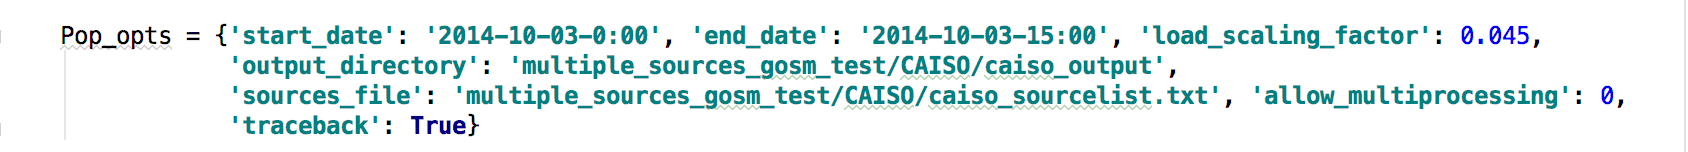
\includegraphics[width=0.9\textwidth]{populator_opts.png}
	\caption{Example of dictionary for populator options.}
\end{figure}

\vspace{10mm}

\item The second dictionary will correspond to options passed into the actual scenario generation process. Again, to learn about every option refer to the documentation. The required options for this dictionary are:
\begin{itemize}
	\item \textbf{use-markov-chains}: Determines if the Markov Chain method is used for generating the scenarios. If this option is set, Markov Chains will be used. (This will be the default method in GOSM 3.0)
	\item \textbf{copula-random-walk}: Determines if copulas are used for the random walk. Can only be set, if use-markov-chains is also set. For multiple sources, this is a must.
	\item \textbf{planning-period-length}: The length for the planning or scenario period as an integer directly following by a capital letter, where "H" stands for hours and "T" stands for minutes.
	\item \textbf{scenario-template-file}: The scenario template file  used for creating the scenarios. For more information look into the User Manual for GOSM 2.0.
	\item \textbf{tree-template-file}: The tree template file used for creating the scenarios. For more information look into the User Manual for GOSM 2.0.
	\item \textbf{reference-model-file}: The reference model which is used for creating the scenarios. For more information look into the User Manual for GOSM 2.0.
\end{itemize}
\begin{figure}[H]
	\centering
	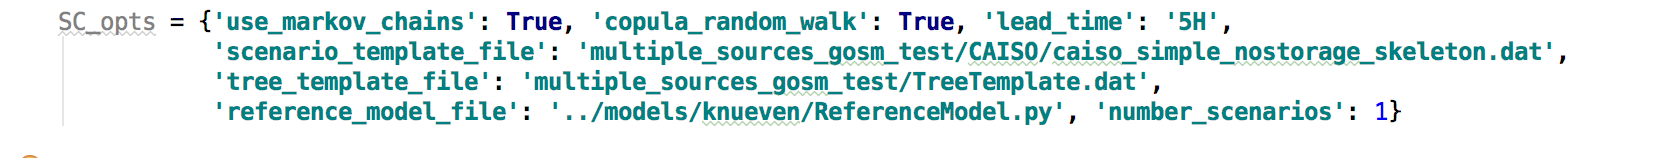
\includegraphics[width=0.9\textwidth]{scenario_creator_opts.png}
	\caption{Example of dictionary for scenario creator options.}
\end{figure}


\end{enumerate}





\end{document}